\chapter{Analysis}
\label{ch:design}
This chapter documents the analysis performed. This is done in order to support the major design decisions in the scope of building a tool that implements the hinting tool concept from \ref{chap:conceptual_design}. It focuses on building models that enable translations from the use case representations to tests -- focusing on broad test coverage. This chapter also presents an execution model that is suitable for translating use case steps to executable source code functions.

\section{Meta model}
\begin{figure}[!htbp]
  \centering
  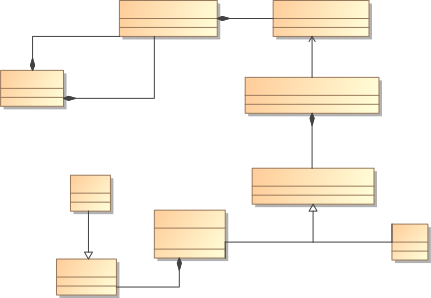
\includegraphics[scale=0.9]{img/3rd_iteration_meta_model}
  \caption{Meta model of the third concept}
  \label{fig:3rd_iteration_meta_model}
\end{figure}
\noindent This section discusses an evolved and simplified version of the meta model introduced in chapter \ref{chap:conceptual_design}, and covers the changes that happened when the model transitioned from concept to design.\medskip

\noindent A central concept that was removed, is the actor actions. While they provided additional information about what actors were capable of, they added little or no value to tests. The predicates that signified the pre- and postcondition needs to be mapped as code in the test templates (see section \ref{sec:technique-overview}). This effectively means that the mapper actor needs write up a function that explicitly break the execution within the conditional steps, in the case of an unmet condition. An example function that realizes this is shown in listing \ref{lst:example-precondition-code} where an \texttt{AssertionError} is thrown if the pre-/postcondition fail.\medskip

\begin{lstlisting}[style=Dart, caption=Example pre-/postcondition code mapping (written manually),label={lst:example-precondition-code}]
void the_user_is_logged_in(User user) {
  if (!user.loggedIn) {
    throw new AssertionError("User is not logged in."); 
  }
}
\end{lstlisting}

\noindent When performing a translation, every use case step will be broken down into a set of decomposed steps. A decomposed step is an \emph{ordered} list of either a definition or just a text. The decomposition is a reversible process, that will be performed by the use of a definition set. A definition set is the information which added by the use case writer and links domain concepts to use cases. Definitions are used to infer which concepts or actors need to passed to the generated test case functions, when performing the use case translation.

\section{Translating a use case}
%GDR
Once we have built the use case models, translation of them is a matter determining which paths they contain and translating them to the test function calls. The signatures of the functions are automatically inferred by the concept types linked in definitions.\medskip

\noindent During the design process, three major constraints for use cases -- in regards to test generation -- were defined. 
\begin{description}
  \item[Steps:] Every step in a use case scenario is a synchronous, self-contained action -- every step must finish before the next starts. Single steps may mutate the system state.
  \item[Termination:] A use case scenario (the main scenario) should always terminate. It should have distinct start and finish. Otherwise, it would be impossible to generate tests from it.
  \item[No extensions nesting:] A design decision that simplified the path determination.
\end{description}
We treat the use case scenario with extensions as a directed graph -- potentially containing cycles. Every node of the graph represents a use case step and every edge the invocation of the next step. An example of a use case graph is shown in figure \ref{fig:use-case-graph}. It consists of a main scenario, which are all the $s_n$ states (state $s_1$ to $s_5$) and an exit point. The exit point is provided to signify explicit termination for the main scenario. Use case extensions that never return to the main scenario, but merely terminate the use case returns directly to this node. The extension node $e_{3.1}$ represent an extension that illustrates this exact behavior.\medskip

\noindent The next subsection goes into more detail on how to extract the different paths from the use case graph.

\begin{figure}[!htbp]
\centering
\begin{tikzpicture}[->,>=stealth',shorten >=0.8pt,auto,node distance=1.8cm,
thick,
extension1 node/.style={circle,fill=blue!20,draw,font=\sffamily\bfseries},
extension2 node/.style={circle,fill=orange!20,draw,font=\sffamily\bfseries},
extension3 node/.style={circle,fill=brown!20,draw,font=\sffamily\bfseries},
exit node/.style={circle,fill=red!20,draw,font=\sffamily\bfseries},
chosen node/.style={circle,fill=green!20,draw,font=\sffamily\bfseries}]

%Scenario
\node[chosen node] (s1) {$s_1$};
\node[chosen node] (s2) [below of=s1] {$s_2$};
\node[chosen node] (s3) [below of=s2] {$s_3$};
\node[chosen node] (s4) [below of=s3] {$s_4$};
\node[chosen node] (s5) [below of=s4] {$s_5$};
\node[exit node] (exit) [below of=s5] {$exit$};

%Extension 1
\node[extension1 node] (e1_1) [left of=s2] {$e_{1.1}$};

%Extension 2
\node[extension2 node] (e2_1) [right of=s4] {$e_{2.1}$};

%Extension 3
\node[extension3 node] (e3_1) [left of=s4] {$e_{3.1}$};

%Paths
\path[every node/.style={font=\sffamily\small}]
(s1)   edge node [] {} (s2)	
(s2)   edge node [] {} (s3)
       edge node [] {} (e1_1)
(s3)   edge node [] {} (s4)
(s4)   edge node [] {} (s5)
       edge node [] {} (e2_1)
       edge node [] {} (e3_1)
(s5)   edge node [] {} (exit)

(e1_1) edge[bend right] node [] {} (s3)
(e2_1) edge[bend right] node [] {} (s2)
(e3_1) edge[bend right] node [] {} (exit)
;
\end{tikzpicture}
\caption{Graph depicting different paths through a use case}
\label{fig:use-case-graph}
\end{figure}
\subsection{Determining paths}
\label{ssec:use-case-paths}
A path of a use case is any graph path that traverses the graph from the initial state $s_1$ to the ($exit$) node. In the simple use case graph in figure \ref{fig:use-case-graph}, we enumerated 11 paths - not counting loops.\medskip

\noindent The basic path of an extension (the one that diverts from the main scenario, and goes straight back to it), once finished can be represented as the union of the path leading in, the path of extension scenario, and the path from the exit point of the extension, to the exit point of the use case represented as a \emph{ordered} set of nodes (\ref{eqn:exten-base-path}). 
\begin{equation}
p_{exten} = \left\lbrace s_1 \dots E_{entry} \right\rbrace \bigcup E_{scenario} \bigcup \left\lbrace E_{entry} \dots exit \right\rbrace
\label{eqn:exten-base-path}
\end{equation}
\noindent Harvesting each additional path ($p_{exten}$) will be a matter of combining the scenario of the use ($E_{scenario}$) with the all the different possible entry and exit paths, as seen in the itemized list above.\medskip

\noindent Once a list of paths is retrieved, it is possible to convert every path, which is essentially a list of active actions either performed by, or affecting, the primary actor. This list will be translated into a test by converting it into code snibblet, and joining them together in a code block that becomes the body of a test function.\medskip

\noindent Until now, the fact that back edges (edges that go backwards in the directed graph) can occur, has been ignored. These edges raise the bar for identifying unique paths, as loops are introduced. Loops are potentially infinite and need to be detected and mapped appropriately.\medskip

\noindent The loop detection is quite simple, if we disallow nested extensions. In that case, the loop detection can be performed solely by detecting that the return point of the extension is not before the entry point in the main scenario. When a loop is detected in an extension, the extension may be flagged as ``looping''.\medskip

\noindent Loops make it impossible to achieve 100\% test coverage, but we could approximate the behavior by defining a fixed number times that the loop must execute and a fixed path that it should always take during the loops. While this is far from optimal, the test generation tool could provide some convenience functions. These should aid the use case writer in choosing which paths should be taken in which loop execution and how many time it should loop. The general use case coverage, however, should be high, as we have the opportunity to generate tests for every possible path.

\section{Mapping the test to the domain}
This section discusses the individual components of a use case with the perspective of converting it into an executable test. In order to write up functions that implement the generated function block stubs in actual system behavior, a programming model is presented in this section.\medskip

\noindent The programming model builds upon the constraint of having the use case represented as an ordered list of steps that are unrolled into paths, that represent the different ways a use case can play out. The steps of these paths need to be executed in order.
\subsection{Step execution}
\label{ssec:step-execution}
\label{sec:use-case-environment}
Executing a test of a given use case path may be considered a long function call-chain. Each new function call passes its computed state onto the next function, which is how variables get passed also. This method of passing along the state is a common pattern in interpreters and compilers, where this state is referred to as ``the environment'', and the state $S_n$ initially fed into the tests with a list of variable and function definitions -- similar to those our meta model. In our test-case compiler we adopt this concept. One of the benefits of this is to have the ability to have an exit procedure that performs state clean upon exit of every use case.\medskip

\noindent An execution of a use case path that consists of $n$ steps could look like the statement in \ref{eqn:path-evaluation}, where every $S_n$, $Precondition$ and $Postcondition$ are all functions taking the mutated environment (the current state) as an argument, returning the environment with the changes they made. Th chain is evaluated right-to-left, and the first function to be called is, thus, the $Precondition$ function.
\begin{equation}
Postcondition \rightarrow S_n \rightarrow S_{n-1} \rightarrow \dotsb \rightarrow S_2 \rightarrow S_1 \rightarrow Precondition \rightarrow env
\label{eqn:path-evaluation}
\end{equation}
The function is applied to the statement, then the result is applied to the matcher which then returns a success or failure value depending on the outcome of the evaluation. For anyone familiar with the concept of monads in functional programming, this concept is quite similar. Here every function carries the state needed by the next function, and forms an execution chain. The model may also be, represented in procedural languages by a list of statements that only operate on input parameters and return their result.\medskip

\noindent An application of this, in a concrete syntax, is shown in listing \ref{lst:example_functional_path}. It shows the nesting of functions in a use case that merely logs in a user, to log it out again. The change is made to the environment and then passed up the call chain to finally be processed by the \textbf{postcondition} function. This approach is very suitable for functional programming languages, as it is functionally pure (assuming each function has no side effects).

\begin{lstlisting}[caption=Example evaluation of a functional call chain,label={lst:example_functional_path}]:
postcondition (
  user_log_out (
    user_log_in (
      precondition (environment)));
\end{lstlisting}

\noindent Alternatively, this can be done in an imperative fashion, using a procedural programming language as shown in listing \ref{lst:example_procedural_path}. The concept of chaining is the same as above, but now the mutated environment is no longer returned, but instead passed implicitly from one statement to the next.

\begin{lstlisting}[caption=Example evaluation of a procedural call chain,label={lst:example_procedural_path}]:
precondition (environment);
user_log_in (environment);
user_log_out (environment);
postcondition (environment);
\end{lstlisting}

\noindent The latter example is the most readable of the two, and the one that maps (visually) the use case steps. It, very explicitly, states which steps are taken for the use case to succeed.

\subsection{Test case environment}
\label{sec:test_case_state}
In order to run the tests, we need to supply them with some input values, which are the actors and domain concept that they need to operate on. These values are inferred by the definitions added to the use case model by the writer of the use case. So, a use case that involves a ``Bookkeeper'' actor needs a pre-built object of that type handed to it by the test environment.\medskip

\noindent Typical test runners use a test model that consist of three basic steps; setup, run and teardown. Setup and teardown are different from pre- and postcondition in that they are unrelated to the test itself. They merely make sure that objects are initialized with right values and, are in the state that the test expects. This fits the need of having to input values to test quite nicely.\medskip

\noindent Assuming that the actor and concept classes that map to the domain model are already written as code, we may use these test runners (or harness) as scaffolding for our test, providing them with the necessary inputs. An example: For the use case ``Send message to contact'' (see appendix \ref{appendix:use-cases}). We need, beforehand, at least a class representing the actor ``Receptionist'' and a class representing a message. Initialization and de-initialization of these objects can then be done by the setup and teardown function of the test runner, respectively.\medskip

\noindent The next obvious question is then; how do we define which objects are available for the test harness? In the test case system, we have made a configuration file that outlines which actors are available, and simply added the data to initial state of the system under test. Another approach could be to turn the creation of resources needed by tests into a use case itself and feed the output of that generated test into the next test. This approach is covered in more detail in the next chapter.

\subsection{Target system state}
\label{ssec:target-system-state}
This sections outlines, from a test runner point of view, a design that -- ideally -- provides a clean view on development system state and how the use cases should mutate it in. It, roughly, re-applies the design from section \ref{ssec:step-execution} on a higher level and encapsulates the (test) system state into an even larger environment.\medskip

\noindent Assuming that the use cases are self-contained\cite{larman2005} in the way that every action and alternative, for a given actor, may be put into a single (large) use case, then it should also be possible to treat use cases as functions that operate on a global system state.\medskip

\noindent Use cases may also specify some expectations to the system state. This is what is defined as preconditions. If we, however, maintain a system state analogy, we may model use case executions as a set of mutation functions that affect the global system state.\medskip

\noindent A simple example: An actor \emph{accountant} has a use case \emph{accountant creates invoice}. This use case requires that the \emph{accountant} actor has previously been created. The creation could be provided by the \emph{admin} actor's \emph{admin creates accountant} use case.\medskip

\begin{figure}[!htbp]
\includegraphics[scale=0.75]{\imgdir system-state-machine-relations}
\centering
\caption{State machine of the perceived system state}
\label{fig:system-state-machine-relations}
\end{figure}

\noindent 
So, the \emph{accountant creates invoice} effectively has a precondition that is provided by \emph{admin creates accountant} to make the global state match what is expected to execute the \emph{accountant creates invoice}. The concept is illustrated in figure \ref{fig:system-state-machine-relations}, where \emph{Use Case 1} is a prerequisite to \emph{Use Case 2}, but \emph{Use Case 3} has no prerequisites. In order to reach completion (termination) and coverage of \emph{Use Case 2}, \emph{Use Case 1} has to be executed.\smallskip

\noindent Each use case state (an example is \textbf{Post-UC1} in figure \ref{fig:system-state-machine-relations}) is a super-state that contains the state space of every alternative scenario. Basically, every node, of every path extracted from the graphs described in section \ref{ssec:use-case-paths} is also a state, and every edge, the mutation function.\medskip

\noindent This model is useful to consider when programming the test support tools and may even be supported by a concept, such as the event stack validation described in appendix \ref{appendix:event-stack-validation}, where the states and transitions are logged and replayed through a set of state machines. But, for the majority of implementations, it should be considered a programming model. Using this model, developers may also chose to build their precondition mappings as other use cases.

\subsection{Simulating error conditions}
\label{ssec:simulating-error-conditions}
%GDR
Use cases may branch out and go to alternatives actions. These branches may signify that an error has occurred, and may be difficult to emulate. Injecting errors in systems to see how they respond to it, is a field of study on its own. For this purpose, some of the failure scenarios could be described as use cases. That is, a sequence of steps that lead up to the error and how the actor experiencing the error must handle it. Simulating error conditions outside of the control of the system under test may be impossible by a mapper. One possible solution is to add an assumption here and merely treat the event or decision as having occurred. An \textbf{assumption} is a no-operation statement that, in some way, must notify the test runner about its occurrence in a test. This may be realized by just injecting a message into the log stream of the use case test.

\section{Technique overview}
\label{sec:technique-overview}
The technique in this thesis may, at this point, be summarized as the following steps:

\begin{enumerate}

  \item Write up use the cases in the tool. This process can be supported by using activity diagrams as a base. This is also covered in section \ref{sec:1st-iteration-test-specification}.
  
  \item When the use cases are written, they need to be annotated using the hinting tool. Each actor and concept role need to be marked as their respective types.
  
  \item When this is done, a template needs to be created. The template should support the individual functions and function stubs with the correct signatures could be generated from the use cases -- once annotated.
  
\item The templates serve a mappings from the use cases to the implemented system and the generation of executable tests from the use cases may now be performed.

\end{enumerate}

Once the tests are generated, they can be checked into a source code repository for a continuous integration service to use or be run locally -- depending on the chosen test runner.\medskip

\section{Summary}
The path coverage, despite the fact that it is a sound concept, does not really scale. For every new extension in the use cases, every test need to be regenerated taking into account this extension. If the system had $n$ paths before, adding a new use case extension, adds an exponential number number of new paths -- especially in the presence of loops. This is very impractical in a development environment with continuously evolving requirements, and can make the running of tests -- because of the large amount of them -- so time consuming that result is useless, once it arrives.\medskip

\noindent
The same basic problem applies to the target system state, and its associated use case mutation functions. If we were to build up complete model for this, it would lead to a state-space explosion very fast.\medskip

\noindent The simplified design of the meta-model does, however, support a more intuitive work-flow, where the use case writer may write up use cases, almost as they would write up use cases normally. The process of this will also described in the next chapter.\medskip

\noindent The implementation discussed in the next chapter will use the meta model introduced in this chapter as its model for use cases. The graph model and path extraction will be implemented, but the test case environment and target system state are left as design patterns for a test mapper to use when writing mappings and test support tools.